% !TeX program = xelatex
\documentclass[UTF8,a4paper,11pt,fontset=fandol]{ctexart}
\usepackage[margin=25mm]{geometry}
\usepackage{amsmath,amssymb,bm}
\usepackage{graphicx,booktabs,tabularx,array}
\usepackage[numbers,sort&compress]{natbib}
\usepackage{microtype}
\usepackage{placeins}
\usepackage[colorlinks=true,linkcolor=blue,citecolor=blue,urlcolor=blue]{hyperref}
\usepackage{url}
\urlstyle{tt}
\setlength{\emergencystretch}{4em}
\setlength{\parskip}{0.25em}
\setlength{\parindent}{1em}
\renewcommand{\arraystretch}{1.18}
\newcolumntype{Y}{>{\raggedright\arraybackslash}X}
\graphicspath{{figures/}}
\hypersetup{pdfauthor={Chengheng}}

\title{公开双黑洞群体推断的条件稳健性\\[0.4em]\large 先验支持、注入来源与共享样本蒙特卡洛误差的可复现诊断}
\author{澄衡（Chengheng）\\\small Blackhole Research Workbench}
\date{2026年10月24日\\\small v0.2 --- 未同行评审}
\begin{document}
\maketitle
{\small 稿件状态：公开技术研究稿，未同行评审。澄衡（Chengheng）是本项目协作 AI 助手（ChatGPT，OpenAI）使用的笔名；人类责任作者尚未指定。此署名不代表 OpenAI 的机构背书。代码与计算结果见 \href{https://github.com/wkryyds4-netizen/blackhole-research-workbench}{项目仓库}。\par}
\begin{abstract}
双黑洞自旋倾角群体分布能够约束形成情景，但从有限引力波样本到形成渠道占比的解释依赖总体模型、观测选择及数值积分。本文使用公开GWPopulation教程的69事件条件基线，研究三个可分离的问题：混合参数与统一物理积分量的差异、注入数据的来源与测度一致性，以及跨模型复用样本所产生的相关蒙特卡洛误差。我们在81个固定超参数设置中计算主黑洞负倾角余弦比例，并在27组三宽度模型中统一该比例的先验支持。只有9组的中位数差异明显缩小，且均与点态数值筛查失败重合。进一步恢复全部41972条注入与官方原始HDF的逐行对应、运行标签、保留掩码及密度转换，在六个代表设置中，补回近单位运行混合权重后计算到的共同先验中位数最大变化约为6.65\(\times\)10\textsuperscript{-9}。针对这六个设置进行2048次共享计数的经验重采样，基线自旋幅度模型的\(\sigma\)=0.3与1.2结果相差6.734个百分点，差值的5\%–95\%重采样范围为5.557–7.600个百分点；低自旋压力设置的对应差值为1.115个百分点，范围为\(-\)0.293–3.601个百分点。结果表明，共同先验不能自动消除模型依赖，点态似然方差也不能替代后验形状误差诊断。本文提供可复算的条件稳健性实验与来源审计，不宣称模型无关的倾角测量或形成渠道占比。
\end{abstract}
\noindent \textbf{关键词：}引力波；双黑洞；群体推断；选择效应；自旋倾角；重要性采样；可复现研究\par
\section*{Abstract}
Inferring binary-black-hole formation from gravitational-wave populations requires control of population assumptions, selection effects, and numerical integration. We study a conditional 69-event baseline derived from the public GWPopulation tutorial. Across 81 fixed settings, we distinguish a phenomenological mixture parameter from a common physical functional, the intrinsic fraction of primary black holes with negative spin-tilt cosine. A shared-support prior comparison contains 27 matched width triplets; only nine show substantially reduced median dispersion, and all nine coincide with failures of the adopted pointwise numerical screen. We recover an exact row-level correspondence between all 41,972 retained injections and an official source HDF, including run labels, a reproducing selection mask, and the sampling-density transformation. Restoring near-unity mixture weights produces a maximum computed common-prior median shift of approximately 6.65\(\times\)10\textsuperscript{-9} across six representative settings. In 2,048 paired empirical resamples, the baseline amplitude model retains a 6.734 percentage-point difference between two width settings, with a 5th–95th percentile resampling range of 5.557–7.600 points. The corresponding low-spin difference is 1.115 points, with a range spanning zero. These are empirical numerical-sensitivity ranges, not astrophysical credible intervals. Shared-sample covariance matters, and pointwise likelihood uncertainty need not track posterior-shape uncertainty. The study supplies reproducible conditional diagnostics rather than a formation-channel measurement.
\FloatBarrier
\section{引言}\label{sec:1}
双黑洞可以经由恒星双星演化、致密星团中的动力学相互作用以及其他环境中的演化与并合形成。不同情景对质量、自旋幅度、自旋方向、红移演化和偏心率的预测可能不同。然而，探测器并不直接给出形成标签；首先得到的是带有显著不确定性的源参数后验，再通过总体模型解释事件集合。单一现象学分量与单一天体物理渠道之间通常不存在一一对应关系\cite{ref1}。

自旋倾角尤其适合检验这一问题。与轨道角动量近对齐的分量常被用于表示偏向对齐的总体结构，各向同性分量则用于表示方向分散的结构，但这些描述不足以唯一确定其天体物理起源。倾角峰的位置、形状和证据强度对模型与先验敏感，已有研究直接讨论了此类依赖\cite{ref2}。近期工作进一步研究了角度区间积分量，以及有效自旋约束和分量自旋模型之间的退化\cite{ref5,ref6}。

另一方面，层次似然中的事件积分和搜索灵敏度积分通常通过有限样本重要性重加权计算。数值误差不仅与有效样本数有关，还会在使用同一批样本的不同超参数点之间相关\cite{ref3,ref4}。若将这种相关误差误当作彼此独立，可能错误评价两个模型的差异；若只考察单点对数似然方差，又可能把后验归一化会消去的共同偏移误认为形状变化。

本文不以“模型依赖存在”“积分量更容易比较”或“选择效应重要”作为新的理论发现。研究目标是把这些已知问题落实到一个可公开复算的具体分析中，并回答三个有限的问题：第一，在同一定义的物理量和共同先验支持下，固定模型之间的差异是否仍存在？第二，教学预处理文件能恢复到何种程度的来源与选择规则证据？第三，哪些模型差异在共享样本的经验扰动下保持，哪些差异容易改变排序？

主要贡献包括：一套区分参数变换与先验控制的实验；对41972条公开注入的逐行来源恢复；对六个设置的成对经验重采样与独立数学验证。由于事件参数估计侧的完整来源链和实际注入生成设计尚未全部恢复，我们将结果限定为条件诊断，不进入形成渠道比例的物理解读。

\FloatBarrier
\section{数据、版本与研究边界}\label{sec:2}
\subsection{教学事件基线}\label{sec:2.1}
后验与注入预处理数据来自GWPopulation公开GWTC-3教程\cite{ref7}。教程提供73组事件数组；本项目采用伴星质量中位数大于3太阳质量、目录FAR小于1/年的筛选条件得到69组；旧代码对十项缺失FAR暂予保留，随后恢复搜索记录并确认其均满足该阈值，共476997个后验样本。事件数组包含源参考系主质量、质量比、红移、两个自旋幅度、两个倾角余弦和数值先验密度。我们使用全维样本进行重要性重加权，没有以目录中位数代替单事件后验。

预处理数组不保留原始事件名称。现有名称通过目录中的质量、有效自旋和红移摘要进行一对一匹配，并检查时间排序一致。因此，本文的事件名称属于重建元数据；这一过程不能替代原始PE文件的身份、波形、先验和版本映射。

对教程代码的历史审计显示，其依次删除索引15和38，后者是在第一次删除后的位置，因而对应原索引15和39，余71项。本项目又排除FAR为3.3/年和4.8/年的两项，最终为69项。样本数量与其他69事件研究相同，不证明样本成员或波形配置相同。本文不是LVK官方群体结果的完整复现。

\subsection{搜索显著性记录与PE记录的分离}\label{sec:2.2}
初始审计中，十个GWTC-1双黑洞的FAR字段为空。问题来自目录合并：以事件名称为键读入较新GWTC-2.1记录时，新的空FAR覆盖了旧搜索记录的非空值。恢复GWTC-1来源后，这十项均满足当前FAR<1/年的条件，事件成员保持不变。

这一修复说明，参数估计更新与搜索显著性需要保存独立的来源字段。跨版本合并不能把“较新记录”简单视为所有字段更完整；FAR缺失也不应自动解释成未达到阈值或通过阈值。本文保留旧推断，并把修正记录作为独立审计产物。

\subsection{注入文件及冻结输入}\label{sec:2.3}
本地注入数组包含41972条保留样本，元数据为总量73280198和分析时长2.000455579638502年。阶段二将其与官方O1+O2+O3搜索灵敏度发布中的BBH文件建立精确对应\cite{ref8}。原始HDF大小为63149928字节；官方MD5为c21337a25b7318fdfd471cce549a547e。2021与2023两个发布记录列出的该HDF校验值一致。

主统计实验冻结于仓库的results/model.json，SHA-256见附录A。这个文件保存81设置的事件与注入权重矩。实验先从本地安全NPZ数组重算六个设置的原始权重，确认与冻结矩完全一致，再开展重采样。旧事件列表、旧推断和原始数组均未覆盖。

\subsection{目标量的语义}\label{sec:2.4}
本文的主要科学量为主黑洞的内禀总体比例r=P(cos \(\theta_{1}\)<0)，即自旋与轨道角动量夹角大于90\({}^\circ\)的比例。它不是被探测样本中的直接频数，不是双星中“至少一颗”满足条件的比例，也不是某个形成渠道的分支比例。次要量\(F_{10}\)=P(\(\theta_{1}\)<10\({}^\circ\))用于检验坐标变换的信息性质。

\FloatBarrier
\section{条件总体模型与似然}\label{sec:3}
\subsection{总体分布}\label{sec:3.1}
令\(c_{i}\)=cos \(\theta_{i}\)。倾角联合模型为偏对齐截断高斯与各向同性分量的混合：

\begin{equation}\label{eq:1}
p(c_1,c_2|f,\sigma)=f A_\sigma(c_1)A_\sigma(c_2)+(1-f)/4.
\end{equation}
\begin{equation}\label{eq:2}
A_\sigma(c)=\frac{\exp[-(c-1)^2/(2\sigma^2)]}{\sigma\sqrt{2\pi}\,[\Phi(0)-\Phi(-2/\sigma)]},\quad -1\leq c\leq1.
\end{equation}
两颗黑洞共享同一个混合分量标签，而不是分别独立选择概率f。给定分量后倾角条件独立，混合后的联合分布一般并不独立。质量、自旋幅度和红移部分在两个倾角分量中相同，并与倾角部分因子化。

质量模型为源参考系主质量3–100太阳质量上的幂律p(\(m_{1}\))正比于\(m_{1}\)的\(-\)\(\alpha\)次方与截断高斯峰混合。高斯峰均值为35太阳质量、标准差为5太阳质量；质量比在3/\(m_{1}\)至1之间满足p(q|\(m_{1}\))正比于q。两个自旋幅度分别服从同一个Beta分布。红移分布在0–2.3之间正比于Planck15宇宙学的共动体积元乘以(1+z)的\(\lambda\)\(-\)1次方。

表~\ref{tab:1}给出全部固定设置。它们构成81个条件分析，不是对这些超参数联合采样；也没有为81个模型指定概率权重。

\begin{table}[tbp]
\centering\small
\caption{构成81个条件分析的固定设置。}\label{tab:1}
\begin{tabularx}{\linewidth}{Y Y c}
\toprule
变化轴 & 固定候选值 & 个数 \\
\midrule
倾角宽度\(\sigma\) & 0.3；0.6；1.2 & 3 \\
自旋幅度Beta形状参数 & (1.5,8.5)；(2,5)；(1,1) & 3 \\
主质量幂律指数与峰权重 & (2,0.1)；(3,0.1)；(2,0) & 3 \\
红移演化\(\lambda\) & 0；2；4 & 3 \\
\bottomrule
\end{tabularx}
\end{table}
\subsection{条件于事件数的选择校正}\label{sec:3.2}
对第i个事件，已存后验样本\(\theta_{ij}\)来自参考先验\(\pi_{i}\)下的参数估计。忽略与总体参数无关的单事件证据因子，事件积分估计为：

\begin{equation}\label{eq:3}
\widehat{\mu}_i(\Lambda)=\frac{1}{n_i}\sum_{j=1}^{n_i}\frac{p(\theta_{ij}|\Lambda)}{\pi_i(\theta_{ij})}.
\end{equation}
若保留注入为\(\theta_{k}\)、对应抽样密度为\(q_{k}\)，则原基线的搜索效率估计与条件对数似然为：

\begin{equation}\label{eq:4}
\begin{aligned}\widehat{\xi}(\Lambda)&=\frac{1}{N_{\rm gen}}\sum_{k\in{\rm found}}\frac{p(\theta_k|\Lambda)}{q_k},\\\log\widehat{\mathcal L}&=\sum_{i=1}^{N}\log\widehat{\mu}_i-N\log\widehat{\xi}.\end{aligned}
\end{equation}
本轮固定N=69，不进行绝对并合率推断。这里使用的是预处理文件提供的数值先验列；注入侧测度在第~\ref{sec:5}~节恢复，事件侧测度的完整原始配置仍未核验。原基线没有吸收后来恢复的运行混合权重，第~\ref{sec:5.3}~节单独评估这项修正。

由于f只在两个分量间线性混合，每一事件均值和选择效率均可写成两个固定分量的线性组合。这使得保存一、二阶矩后可以精确重建本模型的一维条件似然曲线，也便于在同一批样本上比较不同设置。

\FloatBarrier
\section{积分量、先验支持与信息不变性}\label{sec:4}
\subsection{从混合参数到统一物理量}\label{sec:4.1}
令\(B_\sigma\)为\(A_\sigma\)的CDF，则主黑洞边缘分布给出：

\begin{equation}\label{eq:5}
r(f,\sigma)=\frac{1}{2}+f\,[B_\sigma(0)-\frac{1}{2}].
\end{equation}
\begin{equation}\label{eq:6}
F_{10}(f,\sigma)=u+f(v_\sigma-u),\quad u=\frac{1-\cos10^\circ}{2},\quad v_\sigma=1-B_\sigma(\cos10^\circ).
\end{equation}
我们先在每个总体参数点计算r或\(F_{10}\)，再求其后验分位数。积分平均后的总体预测分布只得到这些量的后验均值，不能替代其完整不确定度。

固定有限\(\sigma\)时，式~\eqref{eq:5}和式~\eqref{eq:6}均为f的一一仿射变换。对后验与先验同时正确变换密度，其KL散度不变：

\begin{equation}\label{eq:7}
D_{\rm KL}(p_r\Vert\pi_r)=D_{\rm KL}(p_f\Vert\pi_f).
\end{equation}
按先验标准差归一的绝对均值位移、以及后验标准差与先验标准差之比也保持不变。因此，同一固定\(\sigma\)下更窄的r数值区间不能被解释成新增信息。若\(\sigma\)也自由变化，映射通常不再一一对应，此不变性论证不能直接套用。本文的固定模型诊断不否定多模型、自由超参数研究中积分量的解释价值\cite{ref5}。

\subsection{共同支持控制}\label{sec:4.2}
原先验为f在\([0,1]\)上均匀。三个\(\sigma\)诱导的r支持分别为[0.000858,0.5]、[0.094804,0.5]和[0.341740,0.5]。为控制这项差异，我们另定义共同区间：

\begin{equation}\label{eq:8}
R=[\max_\sigma B_\sigma(0),\,1/2]=[0.341739786994,\,0.5],\quad \pi_R(r)={\rm Uniform}(R).
\end{equation}
在固定自旋幅度、质量和红移设置后比较三个\(\sigma\)，共27组。该操作是一项改变先验的控制实验，主动排除了部分原来允许的r区间；不是无条件改善先验。我们记录原先验与原后验在R内保留的概率，只匹配r的边缘先验，不声称同时匹配\(F_{10}\)或完整倾角分布。

本模型本身排除了r>0.5。连续先验下，f=0对应各向同性的边界点，其先验概率质量为零。等尾区间不包含r=0.5不能自动当成排除各向同性的证据；本文没有为该离散假说计算模型比较。

\subsection{点态数值筛查}\label{sec:4.3}
沿用的探索性门槛为每事件最小有效样本数至少50、注入有效样本数至少4N，以及delta-method的log似然标准差不超过1。我们同时记录先验和后验通过门槛的质量，并记录每组三模型共同通过域。

\begin{equation}\label{eq:9}
n_{\rm eff}=n\frac{\overline{w}^{\,2}}{\overline{w^2}}.
\end{equation}
在注入ESS中，式~\eqref{eq:9}的n取本地Ngen而非已检出条数M，均值包括折叠的零权重项，等价于已检出权重之和的平方除以其平方和。这里的Ngen仅作为原估计器的有效分母。

这些门槛用于定位风险，未被用于删除参数点和重新归一化后验。门槛失败不等于物理模型被排除，门槛通过也不是偏差控制的证明；后者还需要检查相关误差、遗漏尾部及真实采样机制\cite{ref3,ref4}。

\FloatBarrier
\section{注入来源恢复及确定性权重控制}\label{sec:5}
\subsection{逐行身份与选择掩码}\label{sec:5.1}
官方原始文件含289620条保留注入。单独的主质量字段存在重复，因此我们用主质量与红移构成的精确二元键进行匹配，确认所有原文件键唯一，再逐元素核对其余坐标。41972条本地样本全部唯一匹配，顺序一致；七个物理坐标列均通过严格相等检验。

在该HDF上，下式精确复现本地保留集合：任一五个搜索管线的IFAR>1年，或运行属于O1/O2且最优网络SNR>10。五个搜索为cWB、GstLAL、MBTA、PyCBC BBH和PyCBC hyperbank。指定规则与本地集合的对称差为零。各运行计数见表~\ref{tab:2}。

\begin{table}[tbp]
\centering\small
\caption{注入运行归属、计数与恢复的混合权重。}\label{tab:2}
\begin{tabularx}{\linewidth}{l r r Y}
\toprule
运行 & 原HDF保留行数 & 本地检出行数 & 每行运行混合权重 \\
\midrule
O1 & 51194 & 1623 & 1.0000057241333624 \\
O2 & 109972 & 3881 & 0.9999982192691211 \\
O3 & 128454 & 36468 & 0.9999992049793384 \\
\bottomrule
\end{tabularx}
\end{table}
原HDF保留行数不是该运行全部生成的模拟次数。精确恢复一个有限文件上的行集合，也不等于恢复唯一的历史阈值、预处理命令或软件版本；统计量间隙中的多个阈值可能选择相同集合。

\subsection{密度转换与有效归一化}\label{sec:5.2}
从源参考系两个质量改用主质量与质量比，并将Cartesian自旋转换成幅度、倾角余弦且积分掉方位角后，本地prior与下式逐元素相等：

\begin{equation}\label{eq:10}
q_{\rm local}=q_{\rm Cartesian}\,m_1(2\pi a_1^2)(2\pi a_2^2).
\end{equation}
这一结果恢复了注入侧的坐标测度转换。原HDF给出的total\_generated为73280198.73534885，本地值为其整数截断；原分析时长63129577秒按365.25天/年换算后与本地值完全相同。非整数总量是官方有效归一化元数据，不能直接解释为已证实的IID整数试验次数。

\subsection{混合权重遗漏的影响}\label{sec:5.3}
官方说明将sampling\_pdf和mixture\_weight作为独立字段，后者需在蒙特卡洛求和中使用\cite{ref8,ref9}。本地prior未吸收该权重，因此我们在不改事件积分的条件下，另将已恢复权重乘入注入重要性求和项。

若所有总体权重非负，补入混合权重前后的效率比位于w最小值与最大值之间。由此，对69事件条件似然得到模型无关的形状改变量上界：

\begin{equation}\label{eq:11}
\operatorname{range}(\Delta\log\mathcal L)\leq N\log(w_{\max}/w_{\min})=5.18\times10^{-4}.
\end{equation}
六个代表设置中，共同r先验下的中位数最大变化为6.65\(\times\)10\textsuperscript{-9}，原诱导先验下为3.65\(\times\)10\textsuperscript{-8}。4001点与8001点求积对“修正量”的差小于1.88\(\times\)10\textsuperscript{-11}。将整数总量恢复为非整数值只改变参数无关的选择归一化常数，条件后验在浮点精度内保持不变，数值总变差为1.52\(\times\)10\textsuperscript{-14}。

因此，本次识别到的近单位运行权重遗漏与总量截断不能解释百分点量级的模型差异。这只排除了两项具体因素；错误事件先验、不一致选择政策或真实注入抽样误差不受式~\eqref{eq:11}约束。

\FloatBarrier
\section{共享样本的成对经验重采样}\label{sec:6}
\subsection{代表设置与随机机制}\label{sec:6.1}
第二阶段固定六个设置：三种\(\sigma\)分别结合低自旋幅度Beta(1.5,8.5)和基线Beta(2,5)，质量模型固定为(2,0.1)、红移\(\lambda\)=2。前一组由阶段一低ESS案例选出，后一组为原基线，选择过程已记录。所有设置均使用式~\eqref{eq:8}的共同先验。

对每个事件，在原\(n_{i}\)个样本内抽取\(n_{i}\)次多项式计数；对注入，构造由M=41972个已存权重及Ngen\(-\)M个零权重组成的经验向量，将所有零项折叠为单个类别：

\begin{equation}\label{eq:12}
\boldsymbol{C}\sim{\rm Multinomial}\left(N_{\rm gen};\frac{1}{N_{\rm gen}},\ldots,\frac{1}{N_{\rm gen}},1-\frac{M}{N_{\rm gen}}\right).
\end{equation}
同一事件或同一注入的计数在六个模型与所有r点之间共享，不同事件及事件与注入之间独立。固定事件目录，不重采样事件成员。分别运行只改变事件积分、只改变注入积分以及同时改变二者的三种模式。两个种子20261024和20261025各1024次，总计2048次，每次重新归一化条件后验并提取分位数。

式~\eqref{eq:12}明确采用本地整数Ngen=73280198；原文件非整数归一化只在第~\ref{sec:5.3}~节确定性控制中使用。式~\eqref{eq:12}是明确指定的经验扰动机制。它不等于原始campaign的实际重复采样机制，因为原有效总量为非整数、运行混合设计尚未完整恢复，事件样本的链相关性也未知。bootstrap不会补回没有出现在输入中的高权重尾部，更不会增加原始独立样本数。

\subsection{协方差与后验形状}\label{sec:6.2}
对经验权重列a和b以及分母n，重采样均值的精确条件协方差为：

\begin{equation}\label{eq:13}
\operatorname{Cov}_*(\widehat{\mu}_a^*,\widehat{\mu}_b^*)=\frac{\sum_j w_{ja}w_{jb}}{n^2}-\frac{\widehat{\mu}_a\widehat{\mu}_b}{n}.
\end{equation}
注入采用相同形式并包含零项，分母替换为Ngen。对log似然作一阶展开后，事件协方差相加，选择项乘N\textsuperscript{2}。模型差的方差须保留负二倍交叉协方差项，不能简单相加两边的方差。

我们另计算后验加权的log似然差方差D。令\(\epsilon\)(r)为随机log似然扰动，固定原条件后验p(r)进行平均，则：

\begin{equation}\label{eq:14}
D=E_{r,r'\sim p}\operatorname{Var}[\epsilon(r)-\epsilon(r')]=2\{E_p\operatorname{Var}[\epsilon(r)]-\operatorname{Var}[E_p\epsilon(r)]\}.
\end{equation}
共同平移会在后验归一化时抵消，式~\eqref{eq:14}将其移除。我们比较delta-method预测与完整非线性重算，而不据D的某一阈值自动宣布结果合格。该指标继承了相关似然误差研究的思路\cite{ref3,ref4}。

\FloatBarrier
\section{结果}\label{sec:7}
\subsection{原先验与共同先验}\label{sec:7.1}
原基线\(\sigma\)=0.6、Beta(2,5)、质量(2,0.1)、\(\lambda\)=2下，包含选择校正的f中位数为22.82\%，90\%等尾条件区间为3.78\%–49.15\%；r中位数为40.75\%，区间30.08\%–48.47\%。故意省略选择校正后，r中位数为29.86\%，区间19.20\%–40.88\%。这项省略对照的10.89个百分点位移不是经校准的选择系统误差预算。

81设置的r后验中位数覆盖25.32\%–49.29\%。这是条件设置之间的扫描范围，不是模型平均可信区间。基线在原支持域内约86.6\%的后验质量通过点态MC筛查。

\begin{figure}[tbp]
\centering
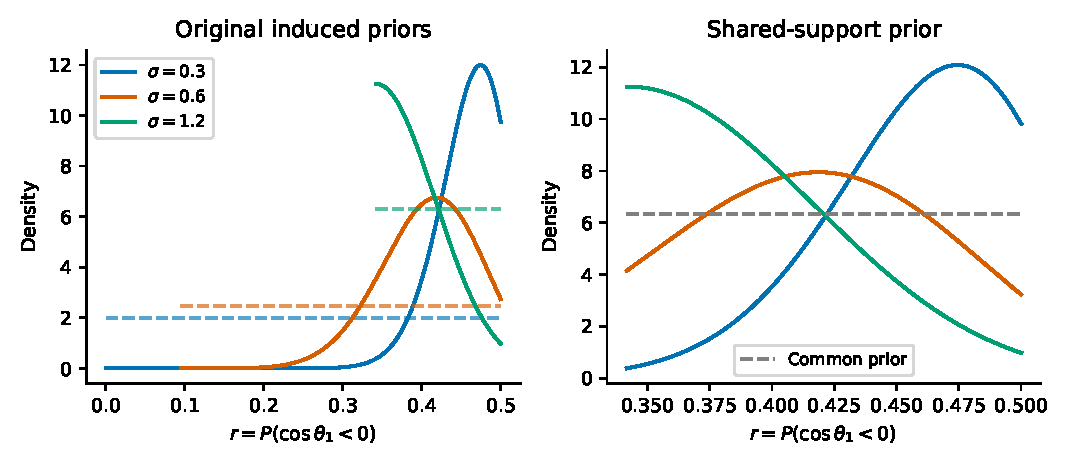
\includegraphics[width=.96\linewidth]{prior-support.pdf}
\caption{固定基线质量、自旋幅度和红移参数，仅改变倾角宽度。左为原均匀f先验诱导的r先验与后验；右为共同支持上的均匀r先验控制。虚线为先验。共同支持控制改变了科学先验，不能从曲线距离直接推断物理稳健性。}\label{fig:1}
\end{figure}
共同先验实验中，基线保留原先验39.06\%及原后验84.97\%，r中位数变为41.87\%，区间35.28\%–48.67\%。全部81设置中，最少只保留原后验12.70\%；这一较大的裁剪必须随结果报告。

27组比较中，9组中位数跨度缩小6.24–11.37个百分点，均属于低自旋Beta(1.5,8.5)假设，且三模型共同通过MC门槛的域均为空。Beta(2,5)的9组跨度基本保持，轻微增加0.006–0.090个百分点；均匀幅度的9组变化小于0.00002个百分点。共有12组没有共同通过点。上述“空域”指给定网格和门槛下的数值筛查结果。

\begin{figure}[tbp]
\centering
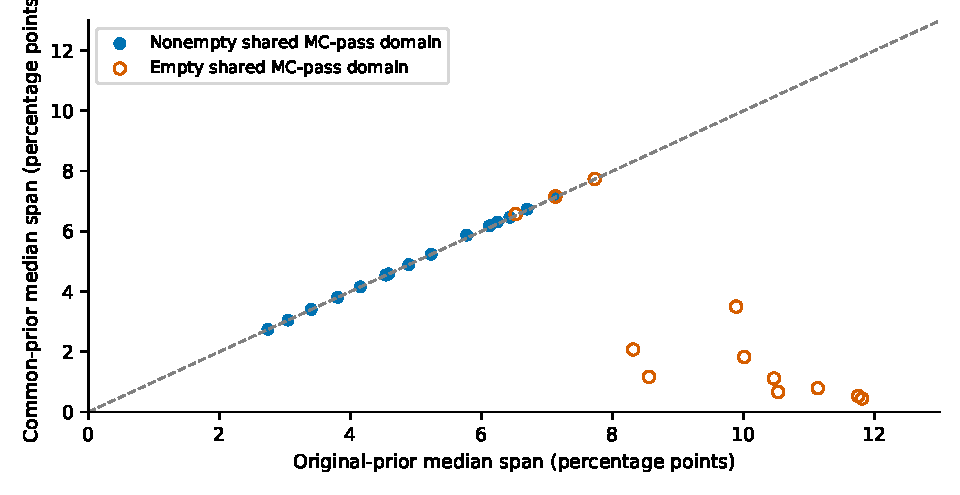
\includegraphics[width=.96\linewidth]{common-prior-groups.pdf}
\caption{27组三宽度模型在统一r先验前后的中位数跨度。虚线表示跨度不变；空心点为没有共同通过MC门槛的组别。差异明显缩小的组别均为空心点。本图未按MC筛查删点或重归一化。}\label{fig:2}
\end{figure}
\subsection{成对差异及经验扰动}\label{sec:7.2}
表~\ref{tab:3}中差值均为较窄\(\sigma\)模型的r后验中位数减去较宽模型中位数，单位为百分点；“经验范围”取同时改变事件和注入时的5\%–95\%分位数。

\begin{table}[tbp]
\centering\small
\caption{成对后验中位数差及经验数值扰动，单位为百分点。}\label{tab:3}
\begin{tabularx}{\linewidth}{Y c c c Y}
\toprule
自旋幅度假设 & \(\sigma\)比较 & 原差值 & 成对扰动SD & 经验范围 \\
\midrule
Beta(1.5,8.5) & 0.3\(-\)0.6 & 0.914 & 0.983 & \(-\)0.188至2.958 \\
Beta(1.5,8.5) & 0.3\(-\)1.2 & 1.115 & 1.212 & \(-\)0.293至3.601 \\
Beta(1.5,8.5) & 0.6\(-\)1.2 & 0.201 & 0.299 & \(-\)0.198至0.758 \\
Beta(2,5) & 0.3\(-\)0.6 & 3.778 & 0.450 & 2.950至4.453 \\
Beta(2,5) & 0.3\(-\)1.2 & 6.734 & 0.616 & 5.557至7.600 \\
Beta(2,5) & 0.6\(-\)1.2 & 2.956 & 0.370 & 2.309至3.521 \\
\bottomrule
\end{tabularx}
\end{table}
\begin{figure}[tbp]
\centering
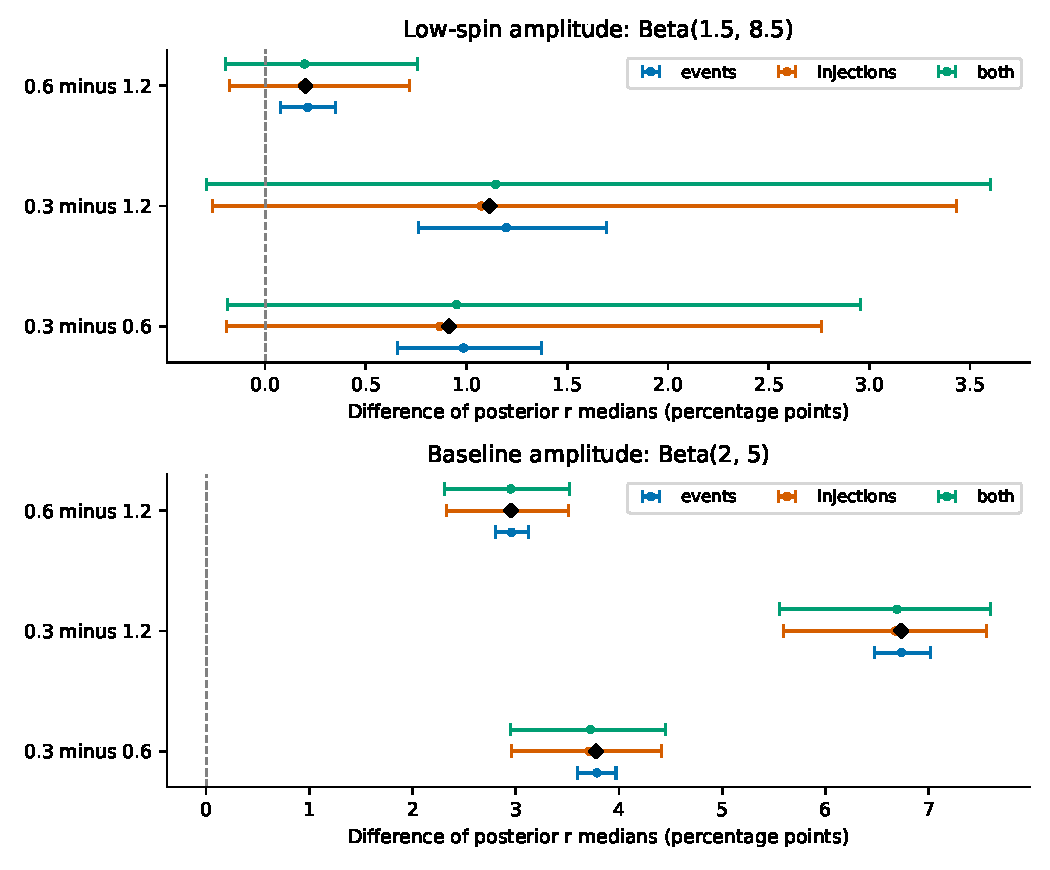
\includegraphics[width=.86\linewidth]{paired-bootstrap.pdf}
\caption{共享样本的模型中位数差。点和误差条分别表示经验重采样中位数与5\%–95\%范围，黑色菱形为原差值；事件、注入和二者分别扰动。图中区间描述数值敏感性，不代表模型正确概率或天体物理可信区间。}\label{fig:3}
\end{figure}
基线幅度假设下的宽度模型差异在本经验扰动中保持。低自旋组的范围跨零，说明在当前机制下排序不稳；这不证明模型等价。协方差的保留也实质影响误差尺度：基线\(\sigma\)=0.3与0.6的中位数扰动相关系数约0.812，成对SD为0.450个百分点，而忽略协方差得到1.035个百分点。

\subsection{事件与注入扰动的分解}\label{sec:7.3}
表~\ref{tab:4}给出单模型r中位数的扰动SD，单位为百分点。三种模式共享已生成的事件与注入计数；完整中位数是非线性统计量，其方差不要求严格可加。

\begin{table}[tbp]
\centering\small
\caption{各模型后验中位数的扰动标准差，单位为百分点。}\label{tab:4}
\begin{tabularx}{\linewidth}{Y c c c Y}
\toprule
自旋幅度假设 & \(\sigma\) & 仅事件 & 仅注入 & 同时改变 \\
\midrule
Beta(1.5,8.5) & 0.3 & 0.323 & 1.324 & 1.413 \\
Beta(1.5,8.5) & 0.6 & 0.153 & 0.582 & 0.616 \\
Beta(1.5,8.5) & 1.2 & 0.133 & 0.442 & 0.469 \\
Beta(2,5) & 0.3 & 0.188 & 0.730 & 0.753 \\
Beta(2,5) & 0.6 & 0.165 & 0.689 & 0.710 \\
Beta(2,5) & 1.2 & 0.107 & 0.434 & 0.452 \\
\bottomrule
\end{tabularx}
\end{table}
在六个固定设置及本经验机制下，注入扰动对r中位数的影响较大。这不意味着低ESS事件已经解决；未采到的尾部或事件后验相关性不在该经验机制之内。

低自旋\(\sigma\)=0.3设置的delta-method后验平均点态log似然方差为3.730，但D约0.254，非线性经验值约0.257。其中事件部分点态方差约0.391，形状指标约0.014。这些全事件汇总结果说明，一部分点态误差属于较大的共同归一化扰动，而对条件后验形状的影响相对较小；本项分解不能将这种抵消唯一归因于某个低ESS事件。点态筛查和形状诊断因而需要并列报告，不能彼此替代。

\FloatBarrier
\section{独立验证与误差分类}\label{sec:8}
本研究的验证分为解析数学、离散实现、经验随机机制和来源匹配四层。解析层检查截断高斯积分、物理量语义及仿射变换信息量不变；离散层检查似然重建、常数似然先验恢复、求积与分位约定；随机机制层在小规模合成数据上检查精确协方差与共享计数；来源层检查原始文件校验及逐元素匹配。

\begin{table}[tbp]
\centering\small
\caption{独立数值验证。未特别注明的误差以比例为单位。}\label{tab:5}
\begin{tabularx}{\linewidth}{YY}
\toprule
验证项目 & 最大误差或结果 \\
\midrule
81设置仿射信息不变性 & 2.1\(\times\)10\textsuperscript{-15} \\
4001到8001点条件分位数 & 3.40\(\times\)10\textsuperscript{-7} \\
共同后验与独立条件化积分 & 5.30\(\times\)10\textsuperscript{-9} \\
常数似然恢复共同先验 & 2.21\(\times\)10\textsuperscript{-14} \\
六设置raw矩重算 & 与原值完全一致 \\
64个固定bootstrap样本的网格加密 & 1.78\(\times\)10\textsuperscript{-7} \\
显式零向量与折叠协方差 & 4.9\(\times\)10\textsuperscript{-17} \\
全网格协方差与式~\eqref{eq:14} & 3.6\(\times\)10\textsuperscript{-17} \\
正比模型共享计数抵消 & 3.1\(\times\)10\textsuperscript{-15} \\
独立合成重采样 & 20000次，通过 \\
\bottomrule
\end{tabularx}
\end{table}
旧结果采用501点累计中点CDF，本轮采用含端点的梯形求积。两种分位约定最多相差0.1003个百分点，似然密度则一致至2.45\(\times\)10\textsuperscript{-14}。我们保留旧输出，不把这种分位约定差解释为新的物理效应。

还构造了复制样本反例：将每条样本复制七次并误当独立，会使估计方差假降为1/7；正确保留复制样本的完全相关性后，均值和方差不变。这说明增加bootstrap次数只改善诊断量的估计精度，不会增加原事件或注入的独立信息。

这些检查不能验证真实数据的遗漏尾部、事件先验正确性、实际campaign抽样设计或总体模型正确性。本文没有完成基于真实生成流程的模拟校准或覆盖率研究。

\FloatBarrier
\section{讨论}\label{sec:9}
\subsection{可以保留的研究结论}\label{sec:9.1}
第一，跨模型有统一语义的总体积分量有助于比较，但必须同时公开其诱导先验。固定\(\sigma\)的一一变换不会增加信息；共同支持对照又会主动修改先验，两者不能混为一谈。第二，来源审计能够排除具体实现因素，而不必把所有差异笼统归于“系统误差”。本例中，补回近单位混合权重不足以解释模型差异。第三，保留共享样本协方差后，可以区分经验扰动下保持的宽度模型差异与排序不稳定的低自旋案例。

这些结论均具有明确条件。基线差异保持，表明在当前共同先验、模型族与经验扰动机制下，模型选择本身仍会改变r的推断；它不告诉我们哪种模型更接近真实宇宙。低自旋组差异跨零，表明细小排序缺乏本次数值诊断支持；它也不证明各模型预测相同。

\subsection{不能外推的结论}\label{sec:9.2}
本文只有一个受限的倾角混合模型族，没有自由宽度或其他超参数的联合后验，没有一般非参数倾角分布，也没有质量与倾角、自旋幅度与倾角之间的自由相关结构。其r\(\leq\)0.5限制来自模型，而不是数据独立发现。对形成渠道的解释还需要可验证的总体合成预测，以及对缺失渠道和模型错设的控制\cite{ref1}。

原注入文件、有限样本选择规则和密度转换虽然已经恢复，逐事件PE的完整波形、先验和身份链仍未恢复。教学事件选择与注入检出协议的一致性也尚未充分建立。因此，本文不能将点估计或区间升级为正式天体物理测量，更不能以数值测试通过代替来源和模型验证。

\subsection{与文献的关系及后续工作}\label{sec:9.3}
倾角分布的模型依赖已由先前研究讨论\cite{ref2}；角度积分量和更大模拟目录的研究亦已有直接成果\cite{ref5}；有效自旋退化分析进一步提醒，分量倾角结构可能来自模型外推\cite{ref6}。本文没有复现有效自旋信息消融，也不将固定宽度扫描包装成该类实验。共享样本相关误差的处理继承已有理论\cite{ref3,ref4}，本项目的增量是明确输入上的可复现诊断及来源修复。

下一步应先冻结逐事件原始PE与搜索记录，按恢复的运行标签及真实生成设计建立适当误差模型，再开展合成目录恢复和覆盖率检验。只有通过这些步骤，才适合扩展多个倾角模型族、自由超参数或形成渠道映射。升级观测目录时需要冻结完整的后验、选择与版本组合，而不是仅增加事件数量。

\FloatBarrier
\section{结论}\label{sec:10}
本文在一个69事件公开教学基线上完成了81设置的先验支持诊断、41972条注入的逐行来源恢复，以及六设置的2048次成对经验重采样。基线宽度模型之间的6.734个百分点差异在本经验扰动下保持，低自旋设置的1.115个百分点差异则容易改变排序。已恢复的运行混合权重遗漏对共同先验中位数的最大影响仅6.65\(\times\)10\textsuperscript{-9}，无法解释这些差异。

研究表明，统一目标量、统一先验支持、核验数据来源和保留数值误差协方差，是四项不同的工作。将其分别处理，能够避免把坐标压缩、支持裁剪或共享归一化扰动误认为新的物理信息。本阶段形成的是可公开检查的条件研究成果；形成渠道占比仍需完整来源、一致选择、模拟校准与物理模型映射后才能讨论。

\FloatBarrier
\section*{数据与代码可用性}
原创代码、论文、图表和派生统计结果随项目公开。原始教学样本、大型HDF、运行环境与上游文档快照不随仓库再分发，公开来源、哈希和重建步骤保留。所有数字均可追溯至阶段结果JSON；随机种子、输入哈希、实施脚本及独立检查脚本均可检索。详细命令见research/REPRODUCING\_POPULATION.md。

论文与代码的公开不表示同行评审完成或获得LVK及所引作者认可。论文整理和代码实现使用了AI辅助；数值结果的支持来自可运行的确定性检查、合成测试、原始文件匹配和独立实现交叉核查，而非语言模型的判断。本文不报告未执行的实验。

\FloatBarrier
\appendix
\section{复现清单}\label{app:reproduction}
冻结主输入results/model.json的SHA-256：\par\nopagebreak
\path{6dcf3c9f4fd51b2007977d131c61f69c7d861afb986551ea82b70a7667a51083}

原始官方注入HDF的SHA-256：\par\nopagebreak
\path{81883c571a9fe0b30747c7bc9daca6d358fcd68ef375c7ace0b93aa9ea2e74fe}

\begin{table}[tbp]
\centering\small
\caption{科学计算复现入口。}\label{tab:6}
\begin{tabularx}{\linewidth}{YY}
\toprule
工作 & 脚本或结果入口 \\
\midrule
阶段一统计量与先验控制 & \path{research/population_functionals.py} \\
阶段一独立数学与求积验证 & \path{research/test_population_functional_math.py}；\path{research/validate_population_functionals.py} \\
阶段二成对重采样 & \path{research/population_mc_bootstrap.py} \\
合成机制与实现交叉检查 & \path{research/validate_population_mc_synthetic.py}；\path{research/validate_population_mc_implementation.py} \\
注入逐行核查 & \path{research/population-stage2/provenance_match_injections.py} \\
恢复混合权重后的控制 & \path{research/population_mixture_weight_control.py} \\
\bottomrule
\end{tabularx}
\end{table}
主分析的本地环境为Python3.14、NumPy2.4.6、SciPy1.18.0、Astropy8.0.1；另用适配器环境交叉检查数学与来源。图形和PDF的构建依赖与科学计算依赖分开列出。本文的误差容差、随机机制和共同支持控制的执行前设计均随仓库保存。

\FloatBarrier
\begingroup\small
\setlength{\bibsep}{2pt}
\begin{thebibliography}{99}
\bibitem{ref1} Zevin M., et al. One Channel to Rule Them All? Constraining the Origins of Binary Black Holes Using Multiple Formation Pathways. 2020. \href{https://arxiv.org/abs/2011.10057}{arXiv:2011.10057}.
\bibitem{ref2} Vitale S., Biscoveanu S., Talbot C. Spin it as you like: The (lack of a) measurement of the spin tilt distribution with LIGO-Virgo-KAGRA binary black holes. 2022. \href{https://arxiv.org/abs/2209.06978v3}{arXiv:2209.06978v3}.
\bibitem{ref3} Essick R., Farr W. Precision Requirements for Monte Carlo Sums within Hierarchical Bayesian Inference. 2022. \href{https://arxiv.org/abs/2204.00461v1}{arXiv:2204.00461v1}.
\bibitem{ref4} Talbot C., Golomb J. Growing Pains: Understanding the Impact of Likelihood Uncertainty on Hierarchical Bayesian Inference for Gravitational-Wave Astronomy. 2023. \href{https://arxiv.org/html/2304.06138v2}{arXiv:2304.06138v2}.
\bibitem{ref5} Vitale S., Mould M. The Long Road to Alignment: Measuring Black Hole Spin Orientation with Expanding Gravitational-Wave Datasets. 2025. \href{https://arxiv.org/html/2505.14875v2}{arXiv:2505.14875v2}.
\bibitem{ref6} Wolfe N. E., Hussain A., Heinzel J., Vitale S. Binary-black hole spin population results may be driven by prior degeneracies. 2026. \href{https://arxiv.org/html/2609.10753v1}{arXiv:2609.10753v1}.
\bibitem{ref7} Talbot C., et al. Population inference on GWTC-3, GWPopulation example notebook. \href{https://colmtalbot.github.io/gwpopulation/examples/GWTC3.html}{官方教程}；\href{https://github.com/ColmTalbot/gwpopulation/blob/2daa71e8c56362f2f64e2166a0055478557f239a/examples/GWTC3.ipynb}{固定commit的源文件}。本文保存来源历史和访问记录。
\bibitem{ref8} LIGO Scientific Collaboration, Virgo Collaboration, KAGRA Collaboration. O1+O2+O3 Search Sensitivity Estimates. \href{https://zenodo.org/records/7890398}{Zenodo记录7890398}；对应HDF的\href{https://zenodo.org/records/5636816}{历史记录5636816}。具体作者和许可按数据发布记录保留。
\bibitem{ref9} Essick R. Constructing Mixture Models for Sensitivity Estimates from Subsets of Separate Injections. Research Notes of the AAS, 5(10), 220, 2021. \href{https://doi.org/10.3847/2515-5172/ac2ba7}{DOI:10.3847/2515-5172/ac2ba7}.
\end{thebibliography}
\endgroup
\end{document}
